\chapter{Complessità computazionale}

\label{Capitolo 2}
Si cerca di catalogare dal punto di vista computazionale i \textbf{problemi
	intrattabili}, ovvero problemi risolvibili ma non in modo \textbf{efficiente}
(ovvero in tempo polinomiale). In alcuni casi si pensa che non esista una
soluzione ma non si hanno dimostrazioni in merito mentre in altri casi è
addirittura dimostrato. Abbiamo quindi delle categorie informali per i problemi:
\begin{itemize}
	\item \textbf{facili}, so risolverli in modo efficiente. È la \textbf{classe P}
	\item \textbf{difficili} o, più formalmente, \textbf{intrattabile}, so
	      risolverli ma non in modo efficiente e non ho una 
	      dimostrazione che mi assicuri che non siano risolvibili in modo efficiente. È
	      la \textbf{classe NP} e la sua sottoclasse \textbf{NP-complete}
	\item \textbf{dimostrabilmente intrattabili}, so risolverli ma so che non esiste
	      un algoritmo efficiente in quanto è stato dimostrato che non può esistere
	\item \textbf{indecidibili}, non so risolverli sempre neanche in modo non
	      efficiente (esiste almeno un input che manda in crisi l'algoritmo ma esiste
	      almeno un caso in cui funzioni)
\end{itemize}
Spesso \textbf{problemi intrattabili} vengono risolti tramite approssimazioni
per arrivare ad una soluzione accettabile anche se non la migliore ma non sempre
è possibile effettuare delle approssimazioni.\\
Anche se avessi ha che fare con un computer mille volte migliore di quelli
attuali, un problema esponenziale avrà comunque tempi non accettabili in
proporzione ad un problema polinomiale. Quindi non sarà il miglioramento
hardware a permettere di rendere accettabile la soluzione di problemi
esponenziali.\\
Come formalismo useremo la \textbf{Macchina di Turing (\textit{TM})},
\textit{deterministica} e \textit{non deterministica}. 
\subsection{Richiami sui grafi}
Analizzeremo in primis
\textbf{problemi sui grafi}. Un grafo è definito come $G=(V,E)$, con $V$ insieme
dei vertici e $E$ insieme degli archi. Un grafo può essere \textit{orientato} o
\textit{non orientato}. Un \textbf{cammino} tra due vertici è una sequenza di
archi che mi porta da un vertice all'altro. Un cammino è detto \textbf{ciclo} se
il vertice sorgente coincide con quello di destinazione. Due vertici sono
\textbf{connessi} se esiste un cammino che li collega. Un \textbf{grafo
connesso} è un grafo dove per ogni coppia di vertici si ha che essi sono
connessi. Se questo cammino è di un solo arco si parla di \textbf{grafo
	completo}, ovvero ogni vertice è \textbf{adiacente} ad ogni altro. Si parla di
\textbf{grafo pesato} se si ha una funzione $W$ che associa un peso ad ogni
arco. \\
\subsection{Richiami sui linguaggi}
Useremo anche la teoria dei linguaggi formali con $V$ alfabeto e stringhe
costruite su $V$. Con $\varepsilon$ abbiamo la stringa vuota e con $V^*$ è
l'insieme di tutte le possibili stringhe costruibili con quell'alfabeto, inclusa
la stringa vuota. $V^*$ è un insieme infinito. Con $V^+$ indico
$V^*/\varepsilon$, ovvero senza la stringa vuota. Un \textbf{linguaggio} $L$ è
un sottoinsieme di $V^*$, quindi $L\subseteq V^*$, che comprende tutti gli
elementi di $V^*$ che seguono una certa \textbf{proprietà} (o più
proprietà). Anche $L$ è un insieme infinito.\\
Un'altra nozione è quella di \textbf{problema}. Un problema computazionale è una
``questione'' a cui si cerca risposta. Più formalmente un problema è specificato
da \textbf{parametri} (l'input del problema) e le \textbf{proprietà} che deve
soddisfare la \textbf{soluzione} (l'output). L'\textbf{istanza} di un problema
specificando certi parametri in input al problema (input che devono essere
coerenti ai parametri richiesti).\\
Cominciamo con degli esempi di problemi comunque risolvibili.
														\section{Complessità parametrica}
														La \textbf{complessità parametrica} è stata introdotta negli anni novanta e
														viene studiata molto in ambito di \textbf{bioinformatica} e studio di
														\textbf{reti/grafi}.\\
														Un problema \textbf{NP-complete} posso dire che alcune istanze sembrano
														risolvibili in tempo polinomiale, fissando determinati parametri che
														caratterizzano l'istanza. Ad esempio prendo \textit{vertex-cover} con al più una
														certa dimensione $k$ in un grafo comunque molto complesso, magari con $10^8$
														nodi e $k$ fissato a un numero piccolo, tipo $5$. Non cerco quindi una minima
														copertura ma una di una certa dimensione, piccola. In questo caso, con $k$
														piccolo, un tempo esponenziale in $k$ è accettabile (esempio $2^5$ è
														accettabile).\\
														Mi serve quindi un algoritmo polinomiale sull'input ma esponenziale su $k$.
														\begin{definizione}
															Un problema decidibile $\Pi$ è \textbf{trattabile fissato il parametro, Fixed
																Parameter Tractable (\textit{FPT})}, con parametro $k$, sse esiste un
															algoritmo $A$, una costante $c$ e una funzione computabile $f$ tale che per
															tutti gli input $\langle x,k\rangle$ $A$ risolve $\Pi$ con tempo di calcolo:
															\[T(n) = f(k)\cdot|x|^c=f(k)\cdot n^c\]
															Si arriva quindi ad un $O(f(k)\cdot n^c)$ con $f$ esponenziale in $k$
															fissato. \\
															L'input diventa quindi $(x,k)$.
														\end{definizione}
														Quindi ho comunque un tempo polinomiale in $x$ ed esponenziale in $k$, $|x|^c\to
														2^k$. Divido quindi l'input in due dimensioni ed esprimo il tempo evidenziando
														i due parametri.\\
														Se avessi un algoritmo $A$, con input $x$, per un problema \textbf{NP-complete}
														avrei $2^{|x|}=2^n$ ma avendo in input $\langle x,k\rangle$ diventa polinomiale
														in $|x|=n$ ma esponenziale in $k$. Nella risposta quindi considero una parte
														limitata dell'input, per questo serve $k$ piccolo.\\
														Fissato $k$ ho una \textbf{soluzione esatta} e quindi gli algoritmi parametrici
														sono vantaggiosi rispetto agli algoritmi di approssimazione.\\
														Non tutti i problemi possono avere un problema parametrico associato.\\
														Queste tecniche vengono usate per trattare problemi \textbf{NP-hard},
														considerando problemi di ottimizzazione e non di decisione.
														\subsection{Vertex-cover parametrico}
														Prendendo \textit{vertex-cover} \textbf{decisionale} cerco una copertura di
														dimensione massima $k$. Ho quindi in input $\langle G=(V,E),k\rangle$ e trovo un
														algoritmo che decide se esiste tale copertura minima in tempo $T(n)$, in
														funzione di $n$ e $k$.\\
														Si ha il seguente definizione:
														\begin{definizione}
															Il problema vertex-cover $(G,k)$ è risolvibile in tempo $O(2^k\cdot |V|)$ dove
															$V$ è l'insieme dei vertici di $G$, con la costante che non dipende da $k$ e
															da $|V|$. Si ha quindi:
															\[O^*(f(x))=O(2^k\cdot |V|)\]
															Avendo $O^*$ che specifica indipendenza da $k$ e da $|V|$.
														\end{definizione}
														Si vuole quindi $s^{|V|}=2^k$.\\
														Si parte quindi cercando di costruire insiemi con al più $k$ vertici esplorando
														un albero binario di ricerca, sviluppandolo fino a profondità $2^k$, che avrà
														come foglie degli insiemi \textit{vertex-cover} di dimensione $k$.\\
														Si quindi ricorre ai \textbf{Bounded search trees (\textit{alberi di ricerca
														limitati})}. Si costruisce quindi un albero binario di profondità $k$, con
														il numero di nodi che quindi cresce circa per $O(2^k)$ e che sono una copertura
														candidata. \\
														Si prende la radice $r$ dell'albero e dato l'arco $(u,v)\in E$ ho due figli di
														$r$, uno con $u$ e l’altro con $v$, costruisco quindi due figli a partire dalla
														radice. Questo si fa in quanto basta avere o $u$ o $v$ nella copertura e quindi
														separo le due situazioni possibili date dalla scelta di uno dei due
														estremi. Scelto un arco arco $(x,v)$ non coperto da $u$ e estendo il nodo di $u$
														collegandolo ad altri due nodi, uno con $\{u, v\}$ e uno con $\{u, x\}$ (fisso
														$k=3$): 
														\begin{center}
															\begin{tikzpicture}[shorten >=1pt,node distance=1.7cm,on grid,auto]
																\node[state, accepting] (q_0) {$r$};
																\node[state] (q_1) [below right=of q_0] {$\{v\}$};
																\node[state] (q_2) [below left=of q_0] {$\{u\}$};
																\path[->]
																(q_0) edge  node {$v$} (q_1)
																(q_0) edge  node [above left] {$u$} (q_2);
															\end{tikzpicture}
														\end{center}
														Proseguo poi via via con ulteriori archi che non sono coperti dai vertici
														foglia, etichettando gli archi dell'albero con l'identificativo del vertice che
														ho aggiunto. \\
														Aggiungo ad esempio $(x,v)$:
														\begin{center}
															\begin{tikzpicture}[shorten >=1pt,node distance=1.9cm,on grid,auto]
																\node[state, accepting] (q_0) {$r$};
																\node[state] (q_1) [below right=of q_0] {$\{v\}$};
																\node[state] (q_2) [below left=of q_0] {$\{u\}$};
																\node[state] (q_3) [below right=of q_2] {$\{u,v\}$};
																\node[state] (q_4) [below left=of q_2] {$\{u,x\}$};
																\path[->]
																(q_0) edge  node {$v$} (q_1)
																(q_0) edge  node [above left] {$u$} (q_2)
																(q_2) edge  node {$v$} (q_3)
																(q_2) edge  node [above left] {$x$} (q_4);
															\end{tikzpicture}
														\end{center}
														aggiungo poi $(z,t)$:
														\begin{center}
															\begin{tikzpicture}[shorten >=1pt,node distance=2.3cm,on grid,auto]
																\node[state, accepting] (q_0) {$r$};
																\node[state] (q_1) [below right=of q_0] {$\{v\}$};
																\node[state] (q_2) [below left=of q_0] {$\{u\}$};
																\node[state] (q_3) [below right=of q_2] {$\{u,v\}$};
																\node[state] (q_4) [below left=of q_2] {$\{u,x\}$};
																\node[state] (q_5) [below right=of q_4] {$\{u,x, z\}$};
																\node[state] (q_6) [below left=of q_4] {$\{u,x,t\}$};
																\path[->]
																(q_0) edge  node {$v$} (q_1)
																(q_0) edge  node [above left] {$u$} (q_2)
																(q_2) edge  node {$v$} (q_3)
																(q_2) edge  node [above left] {$x$} (q_4)
																(q_4) edge  node {$z$} (q_5)
																(q_4) edge  node [above left] {$x$} (q_6)
																; 
															\end{tikzpicture}
														\end{center}
														(mi fermo che sono a $k=3$)\\
														Scriviamo il processo formalmente.\\
														Ricorsivamente si ha che sia $S$ l'insieme che etichetta un vertice, scelgo
														$(u',v')$ in E che non è coperto da S, quindi creo due figli con etichetta $S +
														{u'}$ e $S + {v'}$. Si ha che se c'è un percorso di lunghezza $k$ da $r$ ad un
														nodo $S$ che è una copertura per $G$ allora non c’è bisogno di esplorare oltre
														l’albero, facendo quindi il \textbf{bound}, ovvero il taglio dell'albero. \\
														Ovviamente ogni split non esclude che i due risultati coprano lo stesso
														insieme. La scelta di ordine di archi da esplorare è casuale.\\
														Ovviamente se ad altezza $k$ non trovo una copertura minima significa che non
														esiste una copertura di $k$ nodi.\\
														Vediamo un esempio:
														\begin{esempio}
															Sia dato il grafo:
															\begin{center}
																\begin{tikzpicture}[shorten >=1pt,node distance=2.3cm,on grid,auto]
																	\node[state] (q_0) {$2$};
																	\node[state] (q_1) [below right=of q_0] {$3$};
																	\node[state] (q_2) [below left=of q_0] {$1$};
																	\node[state] (q_3) [below left=of q_2] {$5$};
																	\node[state] (q_4) [below left=of q_1] {$4$};
																	\node[state] (q_5) [below right=of q_1] {$6$};
																	\path[-]
																	(q_0) edge  node {} (q_1)
																	(q_0) edge  node {} (q_2)
																	(q_2) edge  node {} (q_1)
																	(q_2) edge  node {} (q_3)
																	(q_2) edge  node {} (q_5)
																	(q_0) edge  node {} (q_1)
																	(q_1) edge  node {} (q_4)
																	(q_1) edge  node {} (q_3)
																	; 
																\end{tikzpicture}
															\end{center}
															Scelgo di imporre $k=2$.\\
															Inizio con l'arco $(1,2)$ (la scelta è casuale):
															\begin{center}
																\begin{tikzpicture}[shorten >=1pt,node distance=1.7cm,on grid,auto]
																	\node[state, accepting] (q_0) {$r$};
																	\node[state] (q_1) [below right=of q_0] {$\{2\}$};
																	\node[state] (q_2) [below left=of q_0] {$\{1\}$};
																	\path[->]
																	(q_0) edge  node {$2$} (q_1)
																	(q_0) edge  node [above left] {$1$} (q_2);
																\end{tikzpicture}
															\end{center}
															Scelgo poi $(2,3)$:
															\begin{center}
																\begin{tikzpicture}[shorten >=1pt,node distance=1.9cm,on grid,auto]
																	\node[state, accepting] (q_0) {$r$};
																	\node[state] (q_1) [below right=of q_0] {$\{2\}$};
																	\node[state] (q_2) [below left=of q_0] {$\{1\}$};
																	\node[state] (q_3) [below right=of q_2] {$\{1,3\}$};
																	\node[state] (q_4) [below left=of q_2] {$\{1,2\}$};
																	\path[->]
																	(q_0) edge  node {$2$} (q_1)
																	(q_0) edge  node [above left] {$1$} (q_2)
																	(q_2) edge  node {$3$} (q_3)
																	(q_2) edge  node [above left] {$2$} (q_4);
																\end{tikzpicture}
															\end{center}
															scelgo poi $(1,7)$
															\begin{center}
																\begin{tikzpicture}[shorten >=1pt,node distance=2.4cm,on grid,auto]
																	\node[state, accepting] (q_0) {$r$};
																	\node[state] (q_1) [below right=of q_0] {$\{2\}$};
																	\node[state] (q_2) [below left=of q_0] {$\{1\}$};
																	\node[state] (q_3) [below =of q_2] {$\{1,3\}$};
																	\node[state] (q_4) [left=of q_2] {$\{1,2\}$};
																	\node[state] (q_5) [right=of q_1] {$\{2,1\}$};
																	\node[state] (q_6) [below =of q_1] {$\{2,7\}$};
																	\path[->]
																	(q_0) edge  node {$2$} (q_1)
																	(q_0) edge  node [above left] {$1$} (q_2)
																	(q_2) edge  node {$3$} (q_3)
																	(q_2) edge  node [above] {$2$} (q_4)
																	(q_1) edge  node {$1$} (q_5)
																	(q_1) edge  node [left] {$7$} (q_6);
																\end{tikzpicture}
															\end{center}
															e mi fermo essendo a profondità 2.
															Tra le foglie cerco le coperture e noto che $\{1,3\}$ è effettivamente una
															copertura minima.
														\end{esempio}
														\textbf{su elearning appunti extra con algoritmo e calcolo dei tempi}.
														\subsection{TSP metrico}
														\begin{definizione}
															Definiamo \textbf{ciclo di Eulero} come un ciclo che tocca tutti gli archi
															del grafo una e una sola volta. Posso tornare allo stesso vertice e quindi i
															vertici hanno grado entrante pari a quello uscente (numero di archi entranti
															pari a quello di quelli uscenti):
															\[indegree=outdegree\]
														\end{definizione}
														Vediamo quindi un algoritmo parametrico per TSP. Il problema TSP consiste nella
														pratica nel trovare un \textbf{ciclo hamiltoniano} di costo minimo. Ricordiamo
														che un ciclo hamiltoniano è un ciclo semplice, non orientato, che passa per ogni
														nodo di $G$. Il costo del ciclo è pari alla somma dei costi dei suoi archi.\\ 
														Parliamo di \textbf{TSP simmetrico} se il grafo non è orientato, altrimenti è
														detto \textbf{TSP asimmetrico}. TSP è un problema \textbf{NP-hard}.\\
														Studiamo quindi un'euristica per TSP. Si definisce $w_{xy}$ come il peso
														dell'arco tra i nodi $x$ e $y$.\\
														Definiamo \textbf{TSP metrico} come un TSP dove vale la \textbf{distanza}
														``vera'', ovvero i costi sono attribuiti tramite la \textbf{disuguaglianza
															triangolare}. Si ha che $\forall(u,v)\in E$ $w_{uv}=0$ sse $u=v$. Inoltre,
														dati tre nodi distinti, vale appunto la disuguaglianza triangolare:
														\[w_{uv}\leq w_{uz}+w_{zv}\]
														e quindi $w$ introduce una semimetrica, che accettiamo come metrica.
														Applicando questo concetto ad un intero cammino posso dire che un arco tra due
														vertici ha costo sicuramente minore uguale di quello di un cammino tra i due
														archi (praticamente estendo ogni volta il conto facendo una serie di triangoli
														usando sempre la disuguaglianza triangolare).\\
														Una classe molto importante di metriche èquella delle metriche indotte dalle
														varie norme $\norm{\cdot}_p$:
														\[d_{\norm{\cdot}_p}(i,j)=\norm{i-j}_p=\left(\sum_{k=1}^m
															|i_k-j_k|^p\right)^{\frac{1}{p}}\]
															e al variare di $p$ si hanno varie metriche:
															\begin{itemize}
																\item \textbf{distanza di Manahattan} se $p=1$:
																      \[d_{\norm{\cdot}_1}(i,j)=\sum_{k=1}^m|i_k-j_k|\]
																\item \textbf{distanza Euclidea} se $p=2$:
																      \[d_{\norm{\cdot}_2}(i,j)=\left(\sum_{k=1}^m
																      	|i_k-j_k|^2\right)^{\frac{1}{2}}\]
																      	\item \textbf{distanza di Lagrange} se $p=\infty$:
																      	\[d_{\norm{\cdot}_\infty}(i,j)=\max_k\{|i_k-j_k\}\]
																      	\end{itemize}
																      	Per descrivere la 2-approssimazione, detta di \textbf{Christofides}, per TSP
																      	usiamo il ciclo di Eulero.
																      	\begin{definizione}
																      		Definiamo multigrafo come un grafo che prevede la possibilità di avere archi
																      		diversi tra due nodi (possono anche essere cappi).
																      	\end{definizione}
																      	\begin{definizione}[definizione di Eulero]
																      		Un (multi)grafo ammette un ciclo euleriano se e solo se è connesso e ogni nodo
																      		ha grado pari (quindi per un arco entrante ho un arco uscente).\\
																      		Un (multi) grafo connesso e con ogni nodo di grado pari è detto grafo
																      		euleriano. 
																      	\end{definizione}
																      	Esiste un algoritmo polinomiale per costruire un ciclo euleriano da un grafo,
																      	che se lo ammette è chiamato \textbf{grafo euleriano}. Si procede scomponendo il
																      	grafo in cicli che poi vengono fusi secondo un meccanismo che esclude archi già
																      	visitati.\\
																      																	      	
																      	Studiamo quindi l'\textbf{algoritmo di Christofides}. Viene dato in input un
																      	grafo $G=(V,E)$, non orientato, completo, con costi dati dalla funzione $c$ e
																      	dotato di semimetrica. 
																      	L'algoritmo trova un ciclo hamiltonianodi costo al piùdoppio rispetto al ciclo
																      	di costo minimo procedendo tramite alberi di copertura minima, ovvero:
																      	\begin{enumerate}
																      		\item si trova il minimo albero ricoprente $T$ di $G$, questo ha costo
																      		      polinomiale tramite l'\textbf{algoritmo di Prim}. Per questo problema
																      		      l’algoritmo greedy garantisce l’ottimo, basta infatti scegliere gli archi in
																      		      ordine di costo crescente ma saltando quelli che chiudono ciclo
																      		\item si raddoppia ogni arco di $T$ ottenendo un grafo euleriano
																      		\item si costruisce un ciclo euleriano $\epsilon$ di questo grafo, questo ha
																      		      costo polinomiale, basta infatti percorrere uno dopo l’altro tutti i cicli
																      		      ottenuti dai rami dell’albero 
																      		\item si visita $\epsilon$ partendo da un nodo iniziale $u$
																      		\item si costruisce una permutazione $\pi$ dei nodi $V$ di $G$
																      		      \textit{sequenziando i nodi} nell’ordine della loro prima apparizione in
																      		      $\epsilon$ nella visita (potrei avere comunque archi che accorciano il
																      		      percorso essendo $G$ completo (???)). 
																      		\item si restituisce il ciclo hamiltoniano $H$ associato a $\pi$
																      	\end{enumerate}
																      	In pratica si ha un'euristica che si dimostra essere 2-approssimante.\\
																      	Inoltre si ha che $c$ soddisfa la disuguaglianza triangolare (saltando dei nodi
																      	seguo delle scorciatoie) allora si ha che:
																      	\[c(H)\leq c(\epsilon)\]
																      	\begin{definizione}
																      		Sia $H^*$ il ciclo hamiltonianodi costo minimo, e sia $T$ l'albero di
																      		copertura minima di $G$ di costo minimo. Si ha quindi che:
																      		\[c(H^*)\geq c(T)\]
																      	\end{definizione}
																      	\begin{definizione}
																      		Sia $H^*$ il ciclo hamiltoniano di costo minimo, e sia $H$ il ciclo ritornato
																      		dall’algoritmo di Christofides, allora si ha che:
																      		\[c(H)\leq 2\cdot c(H^*)\]
																      		Avendo così la 2-approssimazione.
																      	\end{definizione}
																      	\begin{proof}
																      		Si ottiene quindi che $c(H)$ approssima la soluzione di minimo costo, che
																      		indichiamo con $c(H^*)$, avendo $H^*$ come il ciclo hamiltonianodi costo
																      		minimo. \\
																      		Si ha inoltre che, dato $c(T)$ come costo dell'albero di copertura:
																      		\[c(\epsilon)=2\cdot c(T)\]
																      		perché $\epsilon$ è il ciclo di eulero del grafo $G_T$ ottenuto duplicando gli
																      		archi di $T$ e $\epsilon$ attraversa una sola volta tutti gli archi di tale
																      		grafo:
																      		\[c(\epsilon)=c(\epsilon(G_T))=2\cdot c(T)\]
																      		Si può quindi anche dire che:
																      		\[c(T)\geq c(H^*)\]
																      		dato che $H^*$ è ottenuto da un certo albero $T'$, che non sappiamo se è di
																      		copertura minimo, a cui viene aggiunto un arco $e'$.
																      		Ma sappiamo che:
																      		\[c(T')\geq c(T)\]
																      		riassumendo un ciclo hamiltoniano ottimo è quindi costituito da un albero di
																      		copertura $T'$ (che non sappiamo se è di copertura minimo e quindi $c(T)\leq
																      		c(T')$ più un arco $e'$ che chiude l'albero ad un ciclo per cui: 
																      		\[c(H^*)\geq c(T')\]
																      		avendo che:
																      		\[c(H^*)=C(T')+c(e')\]
																      		A questo punto si ha:
																      		\[c(T)\leq c(T')\leq c(H^*)\]
																      		Sapendo quindi che:
																      		\[c(\epsilon)=2\cdot c(T)\]
																      		e che:
																      		\[2\cdot c(T)\leq 2\cdot c(H^*)\]
																      		e quindi si ottiene che:
																      		\[c(H)\leq c(\epsilon)\leq 2\cdot c(H^*)\]
																      		e quindi:
																      		\[c(H)\leq 2\cdot c(H^*)\]
																      		dimostrando la 2-approssimazione.
																      	\end{proof}
																      																	      	
																      	\begin{esempio}
																      		Partiamo da:
																      		\begin{figure}[H]
																      			\centering
																      			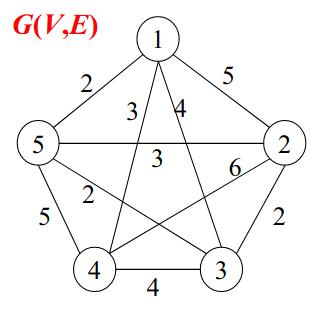
\includegraphics[scale = 0.4]{img/ch1.jpg}
																      		\end{figure}
																      		Procediamo con lo step 1, ottenendo $T$:
																      		\begin{figure}[H]
																      			\centering
																      			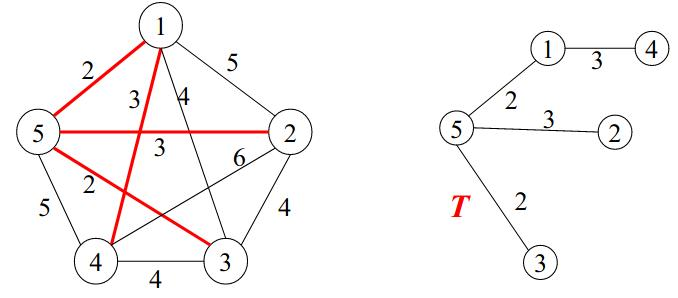
\includegraphics[scale = 0.4]{img/ch2.jpg}
																      		\end{figure}
																      		Procediamo con lo step 2, raddoppiando ogni arco di $T$:
																      		\begin{figure}[H]
																      			\centering
																      			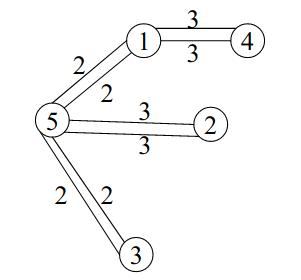
\includegraphics[scale = 0.4]{img/ch3.jpg}
																      		\end{figure}
																      		Procediamo con lo step 3, ottenendo $\epsilon$:
																      		\begin{figure}[H]
																      			\centering
																      			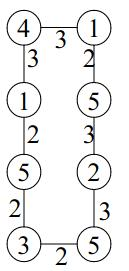
\includegraphics[scale = 0.4]{img/ch4.jpg}
																      		\end{figure}
																      		e con gli step 4 e 5 si ha:
																      		\begin{figure}[H]
																      			\centering
																      			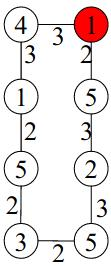
\includegraphics[scale = 0.4]{img/ch5.jpg}
																      		\end{figure}
																      		che deve essere ``letto'' in senso orario.\\
																      		Si ha quindi la sequenza di visita:
																      		\[\epsilon=\{1,5,2,5,3,5,1,4\}\]
																      		con la permutazione associata:
																      		\[\pi=\{1,5,2,3,4\}\]
																      		Si arriva quindi, con lo step 6, a:
																      		\begin{figure}[H]
																      			\centering
																      			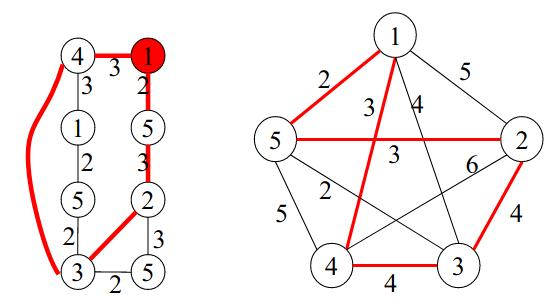
\includegraphics[scale = 0.4]{img/ch6.jpg}
																      		\end{figure}
																      		(avendo che comunque un arco tra due nodi che sostituisce un cammino tra quei
																      		nodi sicuramente costa meno o la più costa uguale, avendo la semimetrica)
																      	\end{esempio}
																      	L'\textbf{algoritmo di Christofides} trova quindi un'euristica cercando un
																      	\textit{lower bound}, tramite l'albero di copertura.\\
																      	\subsubsection{Cammino hamiltoniano e TSP}
																      	Abbiamo visto che il cammino hamiltoniano è un problema \textbf{NP-complete} e
																      	sappiamo che (si veda lezione nel capitolo sulle macchine di Turing,
																      	cronologicamente fatta prima):
																      	\[hamiltonianPath\leq_P TSP\]
																      	(aggiungendo gli archi mancanti con costo maggiore dell'unità)
																      	\begin{definizione}
																      		TSP (non metrico) non ha un'approssimazione costante a meno che $P=NP$.
																      	\end{definizione}
																      	\begin{proof}
																      		Sia $G=(V,E)$ il grafo in analisi su cui costruire il ciclo hamiltoniano.
																      		Costruiamo un
																      		$G'=(V', E', W)$ tale che:
																      		\[
																      			\begin{cases}
																      				w((u,v)) = 1\mbox{ sse } e=(u,v) \in E                            
																      				w(e)=\varepsilon\cdot|V|+1 \mbox{ altrimenti (pesando più di 1)} 
																      			\end{cases}
																      		\]
																      		Si assume quindi  di avere un algoritmo $\varepsilon$-approssimato.
																      		Si hanno due casi:
																      		\begin{enumerate}
																      			\item l'algoritmo restituisce un tour di costo $|V|$ e quindi esiste il
																      			      ciclo hamiltoniano
																      			\item l'algoritmo $A$ restituisce un tour con almeno un arco di costo
																      			      $\varepsilon\cdot|V|+1$ e quindi $A(x)>\varepsilon\cdot |V|$
																      		\end{enumerate}
																      		Ma per definizione di $\varepsilon$-approssimazione ho che:
																      		\[\varepsilon\cdot opt(x)\geq A(x)\]
																      		e quindi si ha che:
																      		\[opt(x)>\frac{A(x)}{\varepsilon}>|V|\]
																      		cioèil tour ottimoèdi costomaggiore di $|V|$ e quindi non esiste un ciclo
																      		hamiltoniano (non c’è modo di avere Un tour di costo $|V|$).\\
																      		Pertanto $A$ diventa un algoritmo per deciderese esiste o meno un
																      		cammino hamiltoniano dove $A$ è polinomiale cioè è nella classe
																      		P. L’algoritmo è fatto come segue:
																      		\begin{itemize}
																      			\item se $A(x)=|V|$ allora ho che $opt(x)=|V|$ ed esiste il ciclo
																      			      Hamiltoniano, altrimenti deve essere che $A(x)>\varepsilon\cdot |V|$ ma per
																      			      costruzione ho che $opt(x)>|V|$ e quindi non esiste il ciclo hamiltoniano ma
																      			      poiché il problema del ciclo hamiltoniano è in NP, ne consegue che P$=NP$,
																      			      dimostrando il definizione.
																      		\end{itemize}
																      	\end{proof}
																      	Esistono quindi problemi che non hanno approssimazione costante.\\
																      	Esistono anche problemi che hanno $\varepsilon$-approssimazione costante
																      	$\forall\,\varepsilon$ piccolo a piacere (si parla di \textbf{Polynomial time
																      		approximation scheme (\textit{PTAS})}). 
																      	\subsection{Closest string}
																      	\textbf{Fatta velocemente e sembra fuori esame}.\\
																      	In questo problema si ha in input una collezione di $k$ stringhe
																      	$s_1,\ldots,s_k$ di lunghezza $l$. Si ha anche un input $d$ e in output si ha
																      	una stringa $s$ tale che:
																      	\[d_H(s,s_j)\leq d,\,\,\,\forall\,j= 1,\ldots,k\]
																      	dove con $d_H(s,s')$ indichiamo la \textbf{distanza di Hamming} tra due stringhe
																      	$s$ e $s'$, ovvero il numero di simboli diversi tra esse.
																      	\begin{definizione}
																      		Closest string è risolvibile in tempo:
																      		\[O(d+1)^d|G|\]
																      		e se $d$ è piccolo, allora il tempo $O(d+1)^d$ è accettabile (esempio per
																      		distanza Hamming $d = 5$) anche quando l’input è molto grande  
																      	\end{definizione}
																      	\textbf{Dimostrazione extra su slide}.